\documentclass[12pt,a4paper]{article}

% --- Bezpatkový font (pdfLaTeX friendly) ---
\usepackage[T1]{fontenc}
\usepackage{nopageno}
\usepackage[utf8]{inputenc}

%img
\usepackage{graphicx}
\graphicspath{ {./img/} }


\IfFileExists{roboto.sty}{
	\usepackage[sfdefault]{roboto}
}{
	\IfFileExists{tgheros.sty}{\usepackage{tgheros}}{\usepackage[scaled=0.94]{helvet}}
}
\renewcommand{\familydefault}{\sfdefault}

% --- Jazyk, vzhled, barvy ---
\usepackage[czech]{babel}
\usepackage[a4paper,margin=2.5cm]{geometry}
\usepackage{microtype}
\usepackage{parskip}
\usepackage{xcolor}
\definecolor{main}{HTML}{004AAD}

% --- Odkazy ---
\usepackage{hyperref}
\hypersetup{colorlinks=true, linkcolor=main, urlcolor=main, citecolor=main}

% --- Grafika ---
\usepackage{graphicx}

% --- Nadpisy ---
\usepackage{titlesec}
\setlength{\parskip}{0.8em}
\setlength{\parindent}{0pt}

% Sekce a podsekce (bez "kapitol")
\titleformat{\section}
{\Large\bfseries\sffamily\color{main}}{\thesection}{0.8em}{}
\titleformat{\subsection}
{\large\bfseries\sffamily\color{main}}{\thesubsection}{0.6em}{}

% --- Obsah (tocloft) ---
\usepackage{tocloft}
\renewcommand{\cfttoctitlefont}{\Huge\bfseries\sffamily\color{main}}
\renewcommand{\cftsecfont}{\color{main}}
\renewcommand{\cftsecpagefont}{\color{main}}
\renewcommand{\cftsubsecfont}{\color{main}}
\renewcommand{\cftsubsecpagefont}{\color{main}}
\renewcommand{\cftdotsep}{1.2}
\renewcommand{\cftsecleader}{\color{main}\cftdotfill{\cftdotsep}}
\renewcommand{\cftsubsecleader}{\color{main}\cftdotfill{\cftdotsep}}

\titleformat{\subsubsection}[runin] % "runin" = inline nadpis (v textu), lze změnit na "hang"
{\sffamily\color{main}}             % styl – sans-serif, modrá
{}                                 % bez čísla
{0pt}                              % mezera mezi číslem (není) a textem
{}                                 % kód před textem

% --- Zápatí s číslem stránky ---
\usepackage{fancyhdr}
\pagestyle{fancy}
\fancyhf{}
\renewcommand{\headrulewidth}{0pt}
\fancyfoot[C]{\thepage}

% --- Meta pro titulní stranu ---
\newcommand{\docTitle}{Název dokumentace}
\newcommand{\docAuthor}{Tvoje společnost}
\newcommand{\docYear}{2025}

% --- Titulní strana ---
\newcommand{\makecleancover}{%
	\begin{titlepage}
		\thispagestyle{empty}
		\centering
		{\color{main}\rule{\textwidth}{2pt}\par}
		\vspace{2.6cm}
		{\fontsize{28pt}{32pt}\selectfont\bfseries\sffamily\color{main}\docTitle\par}
		\vspace{0.8cm}
		{\large\sffamily \docAuthor\par}
		\vspace{0.4cm}
		{\large\sffamily \docYear\par}
		\vfill
		\IfFileExists{logo.pdf}{
			\makebox[\textwidth]{
\includegraphics[width=0.25\textwidth]{logo.pdf}}
		}{
			\IfFileExists{logo.png}{\makebox[\textwidth]{
\includegraphics[width=0.25\textwidth]{logo.png}}{}}
		}
		{\color{main}\rule{\textwidth}{2pt}\par}
	\end{titlepage}
}

% ================== DOKUMENT ==================
\begin{document}
	
	\renewcommand{\docTitle}{Božské tóny v Krušnohoří — Dokumentace produktu}
	\renewcommand{\docAuthor}{ViasWebs}
	\renewcommand{\docYear}{2025}
	
	\makecleancover
	
	% Obsah
	\thispagestyle{empty}
	\tableofcontents
	\clearpage
	
	% Číslování od první sekce (pokud chceš čísla; máš ale \usepackage{nopageno} – ten je vypíná globálně)
	\setcounter{page}{1}
	
	\section{Funkční přehled webu}
	
	\subsection{O projektu}
	Záložka \emph{O projektu} na webu poskytuje uživatelům rychlý vhled do účelu a rozsahu iniciativy. Typicky zde najdou:
	
	\begin{itemize}
		\item \textbf{Stručné představení} — co je projekt \emph{Božské tóny v Krušnohoří} a proč vznikl.
		\item \textbf{Cíle a směřování} — hlavní motivace, zaměření a zapojení regionu.
		\item \textbf{Klíčové aktivity} — výzkumná studie, výstava, kalendář akcí, materiály ke stažení.
		\item \textbf{Pro koho projekt je} — cílové skupiny, zapojení komunit, regionální partnerství.
		\item \textbf{Partnery} — odkazy na jednotlivá místa a zapojené partnery projektu.
	\end{itemize}
	
	\subsection{Aktuality}
	Sekce \emph{Aktuality} zobrazuje chronologicky řazené příspěvky s náhledem
	(titulek, datum, autor) a odkazem na detail. Na úvodní stránce se vybrané
	novinky zobrazují formou karet (\uv{Příspěvky z akcí}).
	
	\subsection{Kalendář akcí}
	Kalendář podporuje zobrazení \textbf{Měsíc/Týden/Den}, navigaci mezi obdobími
	(\uv{Předchozí}, \uv{Dnes}) a filtr kategorií. Nechybí \textbf{Zobrazení pro tisk}
	pro snadnou distribuci programu. V přehledu se zobrazují aktuální měsíce
	a plánované události.
	
	\subsection{Ke stažení}
	Sekce \emph{Ke stažení} slouží pro publikaci dokumentů a materiálů (např. tiskové
	sestavy, podklady pro partnery). Stránka je přístupná z horní navigace a obsah
	je členěn pro snadné stažení.
	
	\subsection{Kontakty a partneři}
	Záložka \emph{Kontakty} poskytuje kontaktní informace; na úvodu je blok
	\emph{Partneři} s logy a odkazy. V patičce je uveden provozovatel a autor designu.
	
	\subsection{Jazyky a sdílení}
	Přepínač \textbf{CS/DE} umožňuje rychlé přepnutí obsahu mezi češtinou a němčinou.
	Na úvodní stránce je také odkaz na \emph{Facebook} pro sdílení a sledování novinek.
	
	\subsection{Cookies a tisk}
	Web zobrazuje informační lištu o cookies s volbou souhlasu.
	U kalendáře je k dispozici speciální \emph{tiskové zobrazení} pro pohodlný export programu.
	
	\newpage
	\section{Technické řešení webu}
	Web je postaven na redakčním systému \textbf{WordPress}, který umožňuje snadnou
	správu obsahu a dlouhodobou udržitelnost. Pro tvorbu vzhledu je využit
	šablonovací systém \textbf{Elementor}, jenž poskytuje vizuální rozhraní pro editaci
	a rychlé sestavování sekcí bez zásahů do kódu. Web je plně \textbf{responzivní}
	(PC, tablet, mobil) a \textbf{lokalizovaný} pro češtinu a němčinu
	(přeshraniční charakter projektu).
	
	\subsection*{Hosting}
	Provoz webu je zajištěn přes hostingovou společnost \textbf{Blueboard}.
	Správu hostingu i souvisejících služeb zajišťuje přímo zákazník.
	
	\newpage
	\section{Wordpress}
	Tento manuál slouží pro základní správu webu postaveného na systému WordPress.
	
	\subsection{Správa účtů a oprávnění}
	WordPress umožňuje více uživatelů s různými oprávněními.
	\begin{enumerate}
		\item \textbf{Přihlášení:} Přes adresu \url{https://bozsketony.cz/wp-admin}
		\item \textbf{Pro zobrazení} uživatelů klikněte v levém menu na položku „Uživatelé“.
	\end{enumerate}

	\begin{figure}[htp]
		\centering
		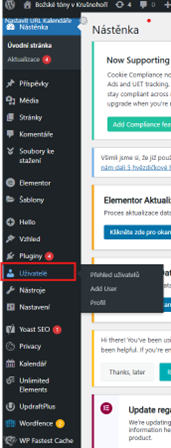
\includegraphics[width=6cm]{role}
		\caption{Ukázka správy rolí ve WordPressu}
		\label{fig:role}
	\end{figure}
	
	\newpage
	Zde můžete upravit, případně vytvořit nové uživatele. Pro přidání uživatele klikněte na „Add User“ a vyplňte požadované údaje ve formuláři.
	
	\subsection{Systémové role}
	Redakční systém WordPress využívá předem definované role. Níže je popis jednotlivých rolí:
	
	\subsubsection*{Administrátor}
	\begin{enumerate}
		\item \textbf{Popis:} Má neomezená práva k celému webu.
		\item \textbf{Práva:} Může instalovat a mazat pluginy a šablony, spravovat uživatele, upravovat nastavení webu a publikovat, editovat či mazat jakýkoliv obsah.
		\item \textbf{Kdy použít:} Role pro majitele webu nebo hlavního správce. Je vhodné mít jen jednoho, maximálně dva administrátory.
	\end{enumerate}
	
	\subsubsection*{Šéfredaktor}
	\begin{enumerate}
		\item \textbf{Popis:} Má plnou kontrolu nad obsahem.
		\item \textbf{Práva:} Může publikovat, upravovat a mazat jakékoliv příspěvky (včetně příspěvků jiných autorů), spravovat rubriky a štítky a moderovat komentáře. Nemůže ale spravovat pluginy, šablony nebo uživatele.
		\item \textbf{Kdy použít:} Ideální pro hlavního editora nebo manažera obsahu, který má na starosti celý publikační plán.
	\end{enumerate}
	
	\subsubsection*{Redaktor}
	\begin{enumerate}
		\item \textbf{Popis:} Může spravovat a publikovat své vlastní příspěvky.
		\item \textbf{Práva:} Může psát, publikovat, upravovat a mazat pouze své vlastní příspěvky. Může také nahrávat soubory (obrázky, dokumenty) a moderovat komentáře ke svým příspěvkům.
		\item \textbf{Kdy použít:} Vhodné pro autory, kteří píší pravidelně a mají právo publikovat svůj obsah bez schválení.
	\end{enumerate}\subsection*{Systémové role}
	Redakční systém WordPress využívá předem definované role. Níže je popis jednotlivých rolí:
	
	\newpage
	\subsubsection*{Administrátor}
	\begin{enumerate}
	\item \textbf{Popis:} Má neomezená práva k celému webu.
	\item \textbf{Práva:} Může instalovat a mazat pluginy a šablony, spravovat uživatele, upravovat nastavení webu a publikovat, editovat či mazat jakýkoliv obsah.
	\item \textbf{Kdy použít:} Role pro majitele webu nebo hlavního správce. Je vhodné mít jen jednoho, maximálně dva administrátory.
	\end{enumerate}
	
	\subsubsection*{Šéfredaktor}
	\begin{enumerate}
	\item \textbf{Popis:} Má plnou kontrolu nad obsahem.
	\item \textbf{Práva:} Může publikovat, upravovat a mazat jakékoliv příspěvky (včetně příspěvků jiných autorů), spravovat rubriky a štítky a moderovat komentáře. Nemůže ale spravovat pluginy, šablony nebo uživatele.
	\item \textbf{Kdy použít:} Ideální pro hlavního editora nebo manažera obsahu, který má na starosti celý publikační plán.
	\end{enumerate}
	
	\subsubsection*{Redaktor}
	\begin{enumerate}
	\item \textbf{Popis:} Může spravovat a publikovat své vlastní příspěvky.
	\item \textbf{Práva:} Může psát, publikovat, upravovat a mazat pouze své vlastní příspěvky. Může také nahrávat soubory (obrázky, dokumenty) a moderovat komentáře ke svým příspěvkům.
	\item \textbf{Kdy použít:} Vhodné pro autory, kteří píší pravidelně a mají právo publikovat svůj obsah bez schválení.
	\end{enumerate}
	
	\subsubsection*{Spolupracovník}
	\begin{enumerate}
	\item \textbf{Popis:} Může psát, ale nemůže publikovat.
	\item \textbf{Práva:} Může psát a upravovat své vlastní příspěvky, ale k jejich publikování je nutné schválení redaktorem nebo administrátorem. Nemůže nahrávat soubory ani spravovat komentáře.
	\item \textbf{Kdy použít:} Skvělé pro externí autory nebo hosty, jejichž příspěvky je potřeba zkontrolovat a schválit před zveřejněním.
	\end{enumerate}
	
	\subsubsection*{Návštěvník}
	\begin{enumerate}
	\item \textbf{Popis:} Standardní role pro nepřihlášeného uživatele, nebo speciálně nastavená role s velmi omezenými právy.
	\item \textbf{Práva:} Obvykle nemá žádná práva k úpravám obsahu. Může pouze číst a komentovat (pokud je to povoleno).
	\item \textbf{Kdy použít:} Role pro každého, kdo navštíví web bez přihlášení. V některých případech se používá i pro přihlášené uživatele, kteří mají právo jen číst exkluzivní obsah.
	\end{enumerate}
	
	\subsection*{Speciální role pro SEO (plugin Yoast SEO)}
	
	\subsubsection*{SEO Manager}
	\begin{enumerate}
	\item \textbf{Popis:} Má plný přístup ke všem funkcím a nastavením pluginu Yoast SEO.
	\item \textbf{Práva a možnosti:}  
	- Úprava globálních nastavení (titulky, meta popisky, RSS, sociální sítě).  
	- Přístup k nástrojům Yoast SEO (editor souborů, přesměrování, import/export).  
	- Ovládání nastavení indexování a crawlingu (noindex, nofollow).  
	- Možnost editovat SEO analýzy všech příspěvků a stránek.  
	- Přístup k pokročilým nastavením (schema markup, integrace s nástroji).
	\item \textbf{Kdy použít:} Ideální pro SEO specialistu, marketingového manažera nebo webmastera.
	\end{enumerate}
	
	\subsubsection*{SEO Editor}
	\begin{enumerate}
	\item \textbf{Popis:} Má omezený přístup, zaměřuje se na optimalizaci obsahu.
	\item \textbf{Práva a možnosti:}  
	- Úprava SEO analýzy a čitelnosti pro vlastní příspěvky.  
	- Nastavení klíčových frází, meta popisků a SEO titulků.  
	- Nemá přístup k globálním ani pokročilým nastavením.
	\item \textbf{Kdy použít:} Vhodné pro autory, redaktory nebo copywritery, kteří optimalizují obsah pro vyhledávače.
	\end{enumerate}
	
	
	\subsubsection*{Spolupracovník}
	\begin{enumerate}
		\item \textbf{Popis:} Může psát, ale nemůže publikovat.
		\item \textbf{Práva:} Může psát a upravovat své vlastní příspěvky, ale k jejich publikování je nutné schválení redaktorem nebo administrátorem. Nemůže nahrávat soubory ani spravovat komentáře.
		\item \textbf{Kdy použít:} Skvělé pro externí autory nebo hosty, jejichž příspěvky je potřeba zkontrolovat a schválit před zveřejněním.
	\end{enumerate}
	
	\subsubsection*{Návštěvník}
	\begin{enumerate}
		\item \textbf{Popis:} Standardní role pro nepřihlášeného uživatele, nebo speciálně nastavená role s velmi omezenými právy.
		\item \textbf{Práva:} Obvykle nemá žádná práva k úpravám obsahu. Může pouze číst a komentovat (pokud je to povoleno).
		\item \textbf{Kdy použít:} Role pro každého, kdo navštíví web bez přihlášení. V některých případech se používá i pro přihlášené uživatele, kteří mají právo jen číst exkluzivní obsah.
	\end{enumerate}
	
	\subsection*{Speciální role pro SEO (plugin Yoast SEO)}
	
	\subsubsection*{SEO Manager}
	\begin{enumerate}
		\item \textbf{Popis:} Má plný přístup ke všem funkcím a nastavením pluginu Yoast SEO.
		\item \textbf{Práva a možnosti:}  
		- Úprava globálních nastavení (titulky, meta popisky, RSS, sociální sítě).  
		- Přístup k nástrojům Yoast SEO (editor souborů, přesměrování, import/export).  
		- Ovládání nastavení indexování a crawlingu (noindex, nofollow).  
		- Možnost editovat SEO analýzy všech příspěvků a stránek.  
		- Přístup k pokročilým nastavením (schema markup, integrace s nástroji).
		\item \textbf{Kdy použít:} Ideální pro SEO specialistu, marketingového manažera nebo webmastera.
	\end{enumerate}
	
	\subsubsection*{SEO Editor}
	\begin{enumerate}
		\item \textbf{Popis:} Má omezený přístup, zaměřuje se na optimalizaci obsahu.
		\item \textbf{Práva a možnosti:}  
		- Úprava SEO analýzy a čitelnosti pro vlastní příspěvky.  
		- Nastavení klíčových frází, meta popisků a SEO titulků.  
		- Nemá přístup k globálním ani pokročilým nastavením.
		\item \textbf{Kdy použít:} Vhodné pro autory, redaktory nebo copywritery, kteří optimalizují obsah pro vyhledávače.
	\end{enumerate}
	
	\subsection{Aktualizace WordPressu a pluginů}
	Pravidelné aktualizace všech dostupných prvků jsou důležité pro bezpečnost a funkčnost webu. Aktualizace doporučujeme provádět pravidelně \textbf{alespoň 1x za měsíc}.
	
	Klikněte na Aktualizovat nyní, pokud je dostupná nová verze 
	
	
	
	
	
	
\end{document}
